\section{Torre de las gallinas}
En secciones anteriores, hemos realizado diversas pruebas con un modelo de un pie sobre un tablero. En esta probaremos los métodos ya implementados con otro modelo que representa una estancia dentro de una torre. Más concretamente, se trata de una parte de la torre de las gallinas, situada en la Alhambra escaneada usando un escáner láser Faro Focus 130. En las figuras \ref{toma1} y \ref{toma2} se muestran las dos tomas que se quieren alinear desde dos puntos de vista diferentes. \\

\begin{figure}[h!]
	\begin{minipage}[b]{0.5\textwidth}
		\centering		
		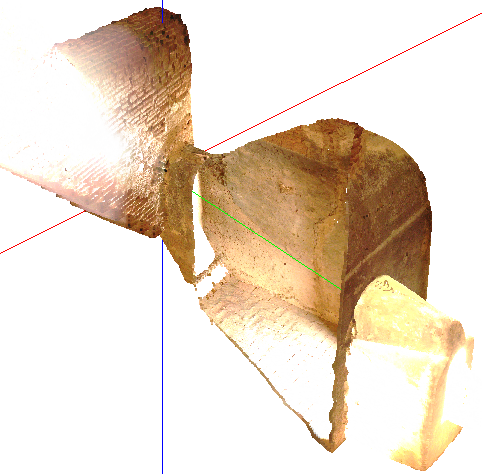
\includegraphics[width=0.8\linewidth]{/Más-ejemplos/me_50_1} 
		%\label{fig:subim1}
	\end{minipage}
	\begin{minipage}[b]{0.5\textwidth}
		\centering
		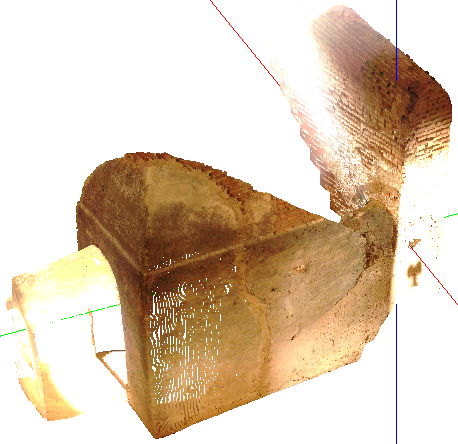
\includegraphics[width=0.8\linewidth]{/Más-ejemplos/me_50_2}
		%\label{fig:subim2}
	\end{minipage}
	\caption{Nube de puntos de la torre de las gallinas usada como toma 1.}
	\label{toma1}
\end{figure}

\begin{figure}[h!]
	
	\begin{minipage}[b]{0.5\textwidth}
		\centering		
		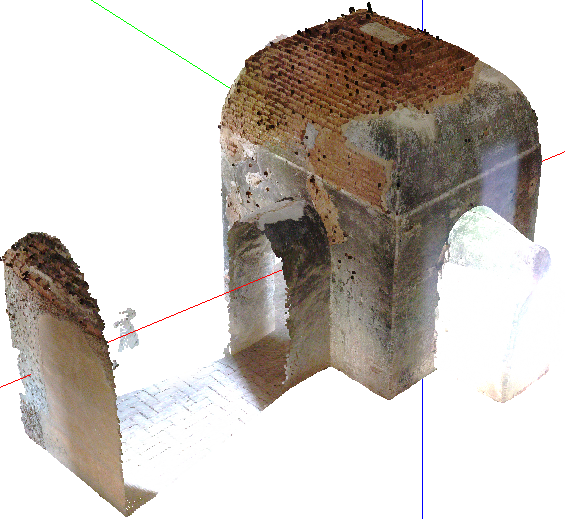
\includegraphics[width=0.8\linewidth]{/Más-ejemplos/me_51_1} 
		%\label{fig:subim1}
	\end{minipage}
	\begin{minipage}[b]{0.5\textwidth}
		\centering
		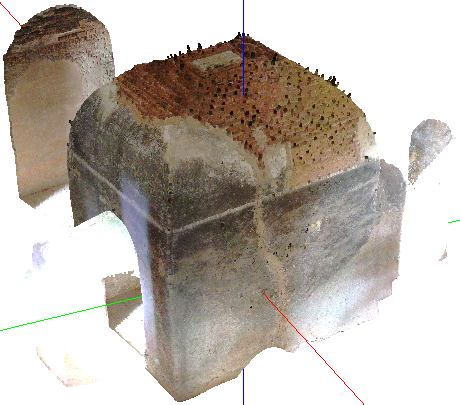
\includegraphics[width=0.8\linewidth]{/Más-ejemplos/me_51_2}
		%\label{fig:subim2}
	\end{minipage}
	\caption{Nube de puntos de la torre de las gallinas usada como toma 2.}
	\label{toma2}
\end{figure}

Destacamos la gran cantidad de puntos que tiene cada una de las nubes: la primera de ellas consta de $ 10\,557\,654 $ puntos y la segunda de $ 10\,801\,863 $ puntos. Si aplicáramos el procedimiento ICP original necesitaríamos bastantes horas para realizar el proceso. Por ello, lo que vamos a hacer es calcular los puntos clave de las tomas y luego aplicamos el algoritmo de alineado a los puntos obtenidos.\\

En primer lugar, vamos a comprobar cómo se compartan las tomas para la obtención de puntos clave sin simplificado y con simplificado tal y como hemos hecho en la sección \ref{varNormal}. También tendremos en cuenta el número de puntos que se detectan en cada una de ellas. El nivel de simplificado que se ha escogido ha sido 5, ya que se ha considerado que puede ser un buen valor para tener la suficiente densidad en la malla y a su vez tener un número de puntos más tratable. Veamos cómo varían los datos de tiempo y tamaño mostrados en la tabla \ref{table:me-normal}. Notamos que se han usado las mismas cotas para el cálculo de los puntos clave que anteriormente.\\

\begin{table}[h!]
	\centering
	\begin{tabular}{| c | c | c |} 
		\hline
		& Original  & Simp. 5 \\
		\hline
		Calc. normales (seg.) & 115.886  &  4.62641\\			 
		Ptos. clave (seg.) & 62.9924 & 2.41946\\
		Ptos. clave (num.) & 862\,225 & 16\,412\\
		\hline
	\end{tabular}
	\caption{Comparación resultados toma 1 original y simplificada (nivel de precisión 5). En la primera columna aparecen los valores que se han medido: tiempo de cálculo en segundos, tiempo en el cálculo de puntos clave y número de puntos clave detectados. En las columnas segunda y tercera aparecen los resultados obtenidos para la toma original y para la simplificada respectivamente.}
	\label{table:me-normal}
\end{table}


\begin{figure}[h!]	
	\begin{minipage}[b]{0.5\textwidth}
		\centering		
		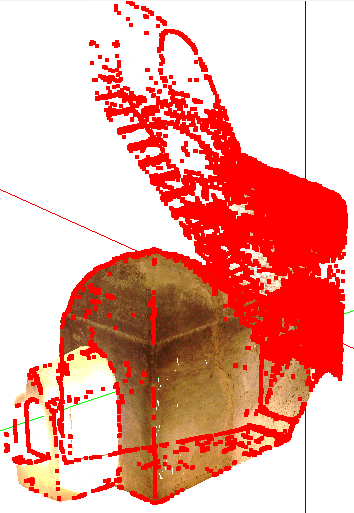
\includegraphics[width=0.7\linewidth]{/Más-ejemplos/me_50_KP_1} 
		%\label{fig:subim1}
	\end{minipage}
	\begin{minipage}[b]{0.5\textwidth}
		\centering
		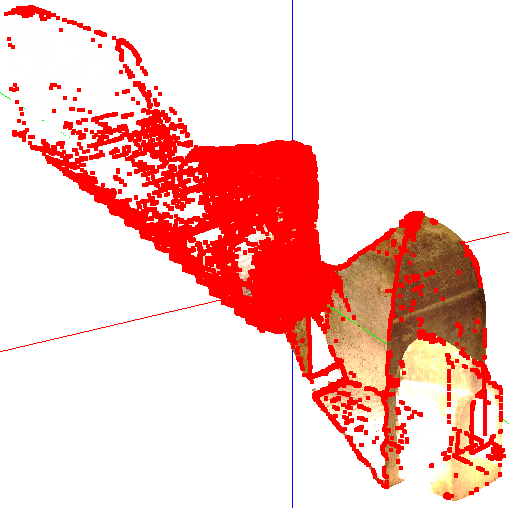
\includegraphics[width=1\linewidth]{/Más-ejemplos/me_50_KP_2}
		%\label{fig:subim2}
	\end{minipage}
	\caption{Puntos clave detectados toma 1 de la torre de las gallinas.}
	\label{me_50_KP}
\end{figure}
\begin{figure}[h!]	
	\begin{minipage}{0.5\textwidth}
		\centering		
		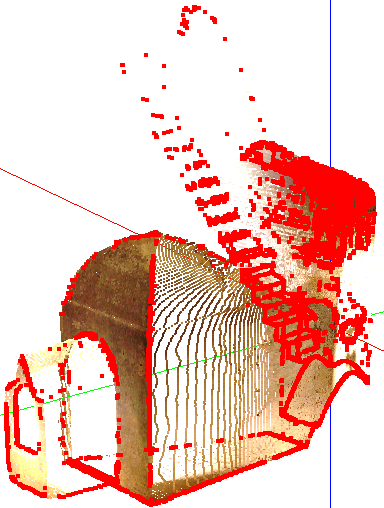
\includegraphics[width=0.7\linewidth]{/Más-ejemplos/me_50_simp5_KP_1} 
		%\label{fig:subim1}
	\end{minipage}
	\begin{minipage}{0.5\textwidth}
		\centering
		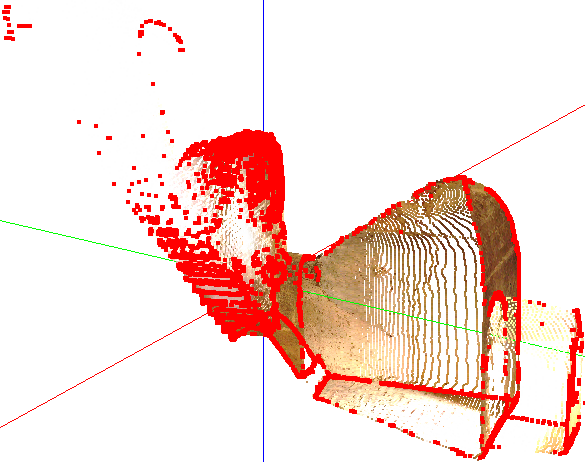
\includegraphics[width=1\linewidth]{/Más-ejemplos/me_50_simp5_KP_2}
		%\label{fig:subim2}
	\end{minipage}
	\caption{Puntos clave detectados toma 1 simplificada (nivel 5) de la torre de las gallinas.}
	\label{me_50_KP_simp4}
\end{figure}

Las imágenes con los puntos clave obtenidos se muestran en \ref{me_50_KP} y \ref{me_50_KP_simp4}. Vemos que a pesar de que en la toma simplificada la densidad de puntos es menor, el algoritmo nuevamente ha sido capaz de identificar mejor las aristas que en la original. Además, se observa que los tiempos empleados para el cálculo de las normales y obtención de puntos clave es considerablemente mejor. Finalmente, en la toma original se han obtenido un total de $ 862\,225 $ puntos lo que sigue siendo un valor demasiado alto para obtener resultados con el algoritmo ICP en un tiempo razonable. Por otro lado, con la versión simplificada hemos obtenido $16\,412 $. Mostramos también los puntos clave de la otra nube de puntos en la figura \ref{me_51_KP_simp4}. Se observa que en la zona superior de la cúpula se han detectado una gran cantidad de los mismos al estar hecha de ladrillo visto. Ahora realizaremos las pruebas del algoritmo comparando los valores del descriptor para la obtención de los puntos clave, ya que, en el ejemplo del pie anterior hemos observado que tardaba menos en la ejecución de cada iteración que viendo el número de ceros de los productos escalares. \\

\begin{figure}[h!]	
	\begin{minipage}[b]{0.5\textwidth}
		\centering		
		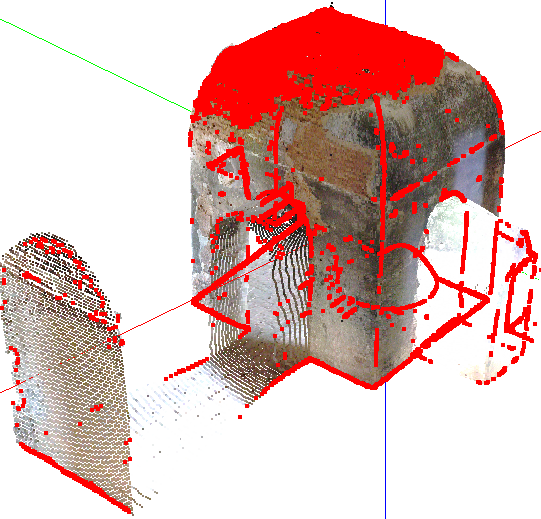
\includegraphics[width=0.75\linewidth]{/Más-ejemplos/me_51_simp5_KP_1} 
		%\label{fig:subim1}
	\end{minipage}
	\begin{minipage}[b]{0.5\textwidth}
		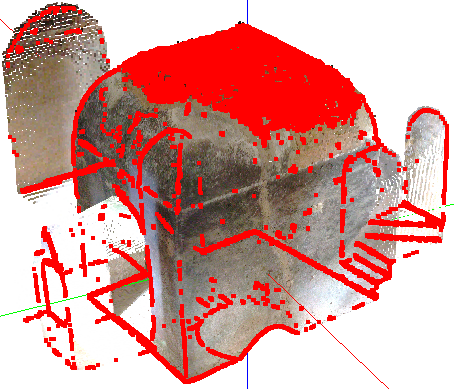
\includegraphics[width=0.8\linewidth]{/Más-ejemplos/me_51_simp5_KP_2}
		%\label{fig:subim2}
	\end{minipage}
	\caption{Puntos clave detectados toma 2 simplificada de la torre de las gallinas. Se han detectado un total de $ 33\,187 $ puntos.}
	\label{me_51_KP_simp4}
\end{figure}

En la figura \ref{fig:ICPtorrePre} aparecen las tomas tras el prealineado y en la \ref{fig:ICPtorre} mostramos los pasos del proceso aplicando el algoritmo entre puntos clave. \\

\begin{figure}[h!]	
	\begin{minipage}[b]{0.5\textwidth}
		\centering		
		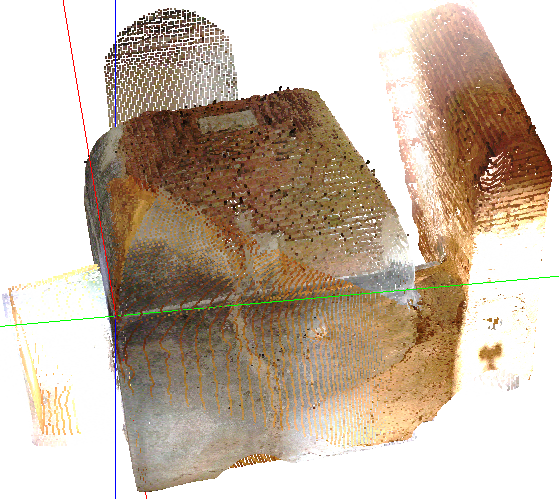
\includegraphics[width=0.7\linewidth]{/Más-ejemplos/me_pre_1} 
		%\label{fig:subim1}
	\end{minipage}
	\begin{minipage}[b]{0.5\textwidth}
		\centering
		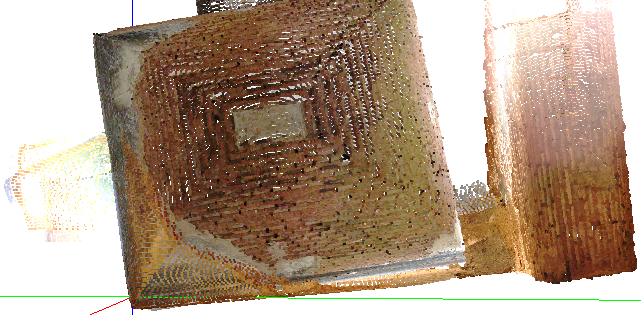
\includegraphics[width=1\linewidth]{/Más-ejemplos/me_pre_2}
		%\label{fig:subim2}
	\end{minipage}
	\caption{Vista general y detalle del prealineado de las tomas de la torre de las gallinas.}
	\label{fig:ICPtorrePre}
\end{figure}

\begin{figure}[h!]	
	\begin{minipage}[b]{0.5\textwidth}
		\centering		
		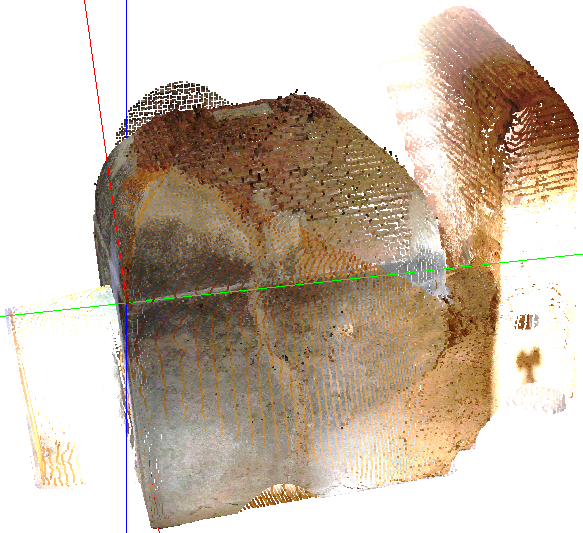
\includegraphics[width=0.7\linewidth]{/Más-ejemplos/me_pru1_it1_1} 
		%\label{fig:subim1}
	\end{minipage}
	\begin{minipage}[b]{0.5\textwidth}
		\centering
		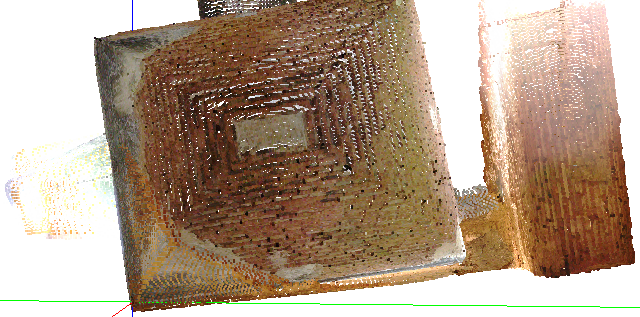
\includegraphics[width=1\linewidth]{/Más-ejemplos/me_pru1_it1_2}
		%\label{fig:subim2}
	\end{minipage}
	\begin{minipage}[b]{0.5\textwidth}
		\centering		
		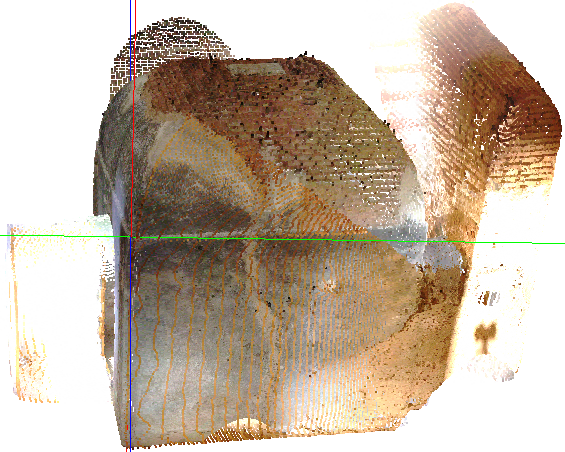
\includegraphics[width=0.7\linewidth]{/Más-ejemplos/me_pru1_it4_1} 
		%\label{fig:subim1}
	\end{minipage}
	\begin{minipage}[b]{0.5\textwidth}
		\centering
		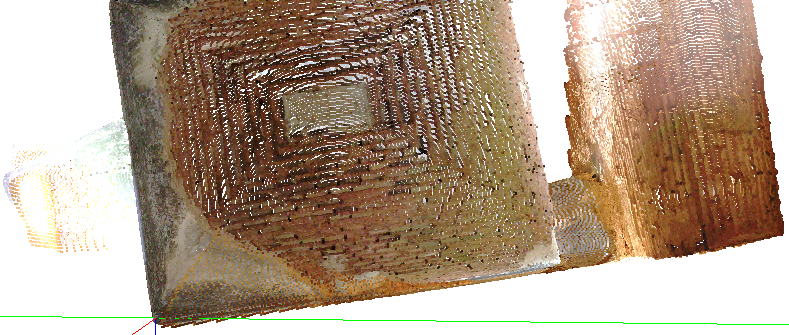
\includegraphics[width=1\linewidth]{/Más-ejemplos/me_pru1_it4_2}
		%\label{fig:subim2}
	\end{minipage}
	\caption{Dos vistas con el resultado de la primera iteración (fila superior) y de la cuarta iteración (fila inferior).}
	\label{fig:ICPtorre}
\end{figure}

\begin{comment}
EN los segundos me salía entorno a 17!!!! con cota unos 0.003
\end{comment}

\begin{table}[h!]
	\centering
	\begin{tabular}{| c | c | c | c | c |} 
		\hline
		It. & Dist. antes (mm) & Dist. después (mm) & Segundos & Num. puntos \\
		\hline
		1 &  206.0735 & 203.3742 & 40.4705 & 1\,997 \\				  
		2 & 185.7078 & 179.6215 & 41.7012 & 2\,219  \\	
		3 & 184.4570 & 182.8958  & 41.8810 &  2\,385 \\
		4 & 182.9830 &  184.7062 & 35.8616 & 2\,473\\
		\hline
	\end{tabular}
	\caption{Resultados ajuste mediante ICP de la torre de las gallinas usando puntos clave. En la primera columna aparece el número de cada iteración en la segunda y tercera las distancias medias antes y después de cada iteración respectivamente. En la cuarta se incluye el tiempo en segundos que ha tardado cada iteración y en última columna el número de puntos clave de la primera toma con ``correspondencia'' en la segunda.}
\end{table}

Vemos cómo el método ha funcionada correctamente a la hora de hacer corresponder el hueco en la pared que se encuentra a la izquierda y cuadrar las paredes de la habitación. Recordamos que el alineado obtenido no es el más refinado, ya que en caso de quererlo deberíamos usar todo el modelo. Finalmente, destacamos que en el último paso, la distancia ha aumentado tras el procedimiento lo que puede parecer contradictorio. Sin embargo, en ocasiones se ha visto en la práctica que el método cuando está cerca de la solución óptima empieza a oscilar. Además,  en las pruebas que estamos realizado no tenemos en cuenta un criterio de parada en función de la variación de la distancia media obtenida. Por último, también vemos que el número de puntos clave a los que se le aplica el método no es el mismo en cada caso. Por ello, entre una iteración y otra no es raro que aumente la distancia media. En lo relativo al número de puntos clave, vemos que ha ido aumentando en cada paso por lo que las tomas están cada vez ``más cerca''.

\section{Sensibilidad y uso en prealineado}
En la sección anterior, hemos usado los puntos clave para alinear dos tomas. En el ejemplo, tras el prealineado dichas tomas estaban ``bien'' posicionadas, es decir, lo suficientemente cerca la una de la otra para asegurar en todo lo posible que el algoritmo funcionase correctamente. Nos hacemos ahora las siguientes preguntas: ¿cómo de sensible es el método propuesto a la alineación inicial? o ¿se podría usar para el propio prealineado?. La primera no es una cuestión baladí, ya que, como se ha indicado anteriormente, es un paso crucial. Si a dos nubes de puntos, se le aplica el procedimiento general ICP no podemos asegurar que si repetimos el proceso con otro prealineado  también funcione. Con esta sección, pretendemos determinar cómo de bien posicionadas deben de estar las tomas. Cuanto menos sensible sea, menos nos debemos de preocupar del mismo e incluso si le afecta poco, podríamos usarlo sin necesidad de prealineado. Destacar que el objetivo de esta sección no es el análisis del tiempo que tarda en ejecutarse el algoritmo por lo que no se incluirán dichas tablas como en anteriores ejemplos.\\

De este modo, volvemos a las tomas que usamos anteriormente y se muestran en las figuras \ref{toma1} y \ref{toma2}. Si aplicamos el procedimiento a las muestras tomadas directamente desde el escáner sin ningún prealineado obtenemos la secuencia de la figura \ref{fig:sensi-1}. Destacar que se ha quitado el límite de longitud máxima para considerar el mínimo. De otro modo, los puntos clave más alejados no se tendrán en cuenta. \\

\begin{figure}[h!]	
	\begin{minipage}[b]{0.5\textwidth}
		\centering		
		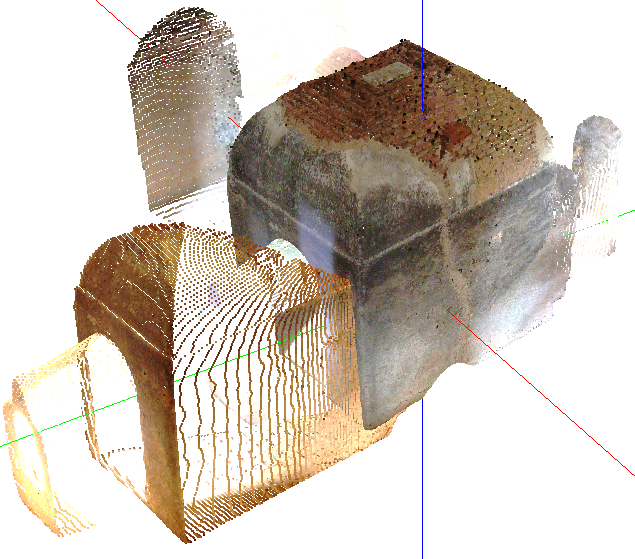
\includegraphics[width=0.8\linewidth]{/Más-ejemplos/sens-1_0} 
		%\label{fig:subim1}
		\caption*{Situación inicial.}
	\end{minipage}
	\begin{minipage}[b]{0.5\textwidth}
		\centering
		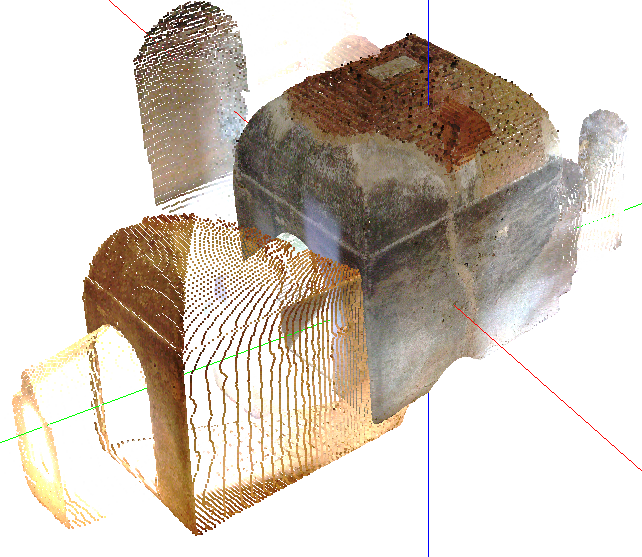
\includegraphics[width=0.8\linewidth]{/Más-ejemplos/sens-1_1}
		%\label{fig:subim2}
		\caption*{Tras una iteración.}
	\end{minipage}
	\begin{center}
		\begin{minipage}[b]{0.5\textwidth}
		\centering		
		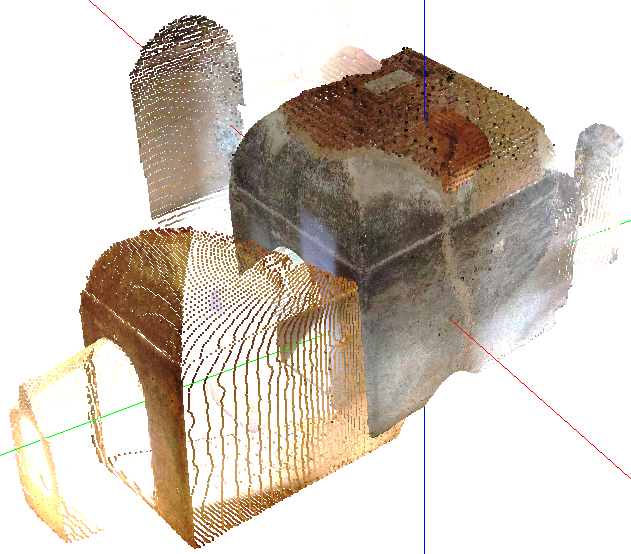
\includegraphics[width=0.8\linewidth]{/Más-ejemplos/sens-1_2} 
		%\label{fig:subim1}
		\caption*{Tras dos iteraciones.}
	\end{minipage}
	\end{center}
	\caption{Ejemplo de sensibilidad. Aplicación del algoritmo ICP sin prealineado.}
	\label{fig:sensi-1}
\end{figure}

Vemos que el resultado no ha sido satisfactorio al no haber prácticamente cambios en el modelo. Esta situación puede deberse en cierta medida a que en la primera nube, se centran los puntos clave en la zona de la escalera y en la segunda, en la cúpula. Observamos que dichas zonas están juntas por lo que intenta ajustar esas zonas. Utilizamos ahora un prealineado no demasiado exacto para ver cómo se comporta el método.  A partir de ahora, sí utilizaremos la cota para aceptar el mínimo. Esta se basará en un valor aproximado a la distancia entre los terceros vértices del prealineado ya, que de ese modo obtenemos cierta referencia de las distancia, que manejamos. Claramente, este valor debe ser mayor, ya que las tomas están más separadas lo que también conllevará que se incremente el tiempo de cómputo. Los resultados aparecen en las figuras \ref{fig:sensi-2-1}, \ref{fig:sensi-2-2} y \ref{fig:sensi-2-3}.\\

\begin{figure}[h!]	
	\begin{minipage}[b]{0.5\textwidth}
		\centering		
		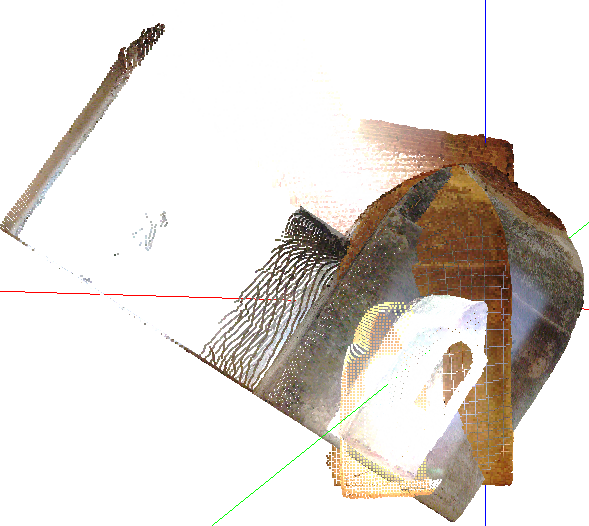
\includegraphics[width=0.7\linewidth]{/Más-ejemplos/sens-3_01} 
		%\label{fig:subim1}
	\end{minipage}
	\begin{minipage}[b]{0.5\textwidth}
		\centering
		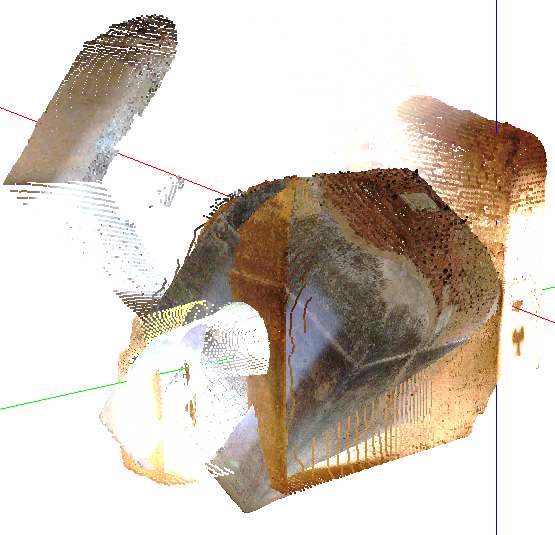
\includegraphics[width=0.7\linewidth]{/Más-ejemplos/sens-3_02}
		%\label{fig:subim2}
	\end{minipage}	
	\caption{Situación inicial. Usamos un prealineado no exacto.}
	\label{fig:sensi-2-1}
\end{figure}
\begin{figure}[h!]	
	\begin{minipage}[b]{0.5\textwidth}
		\centering		
		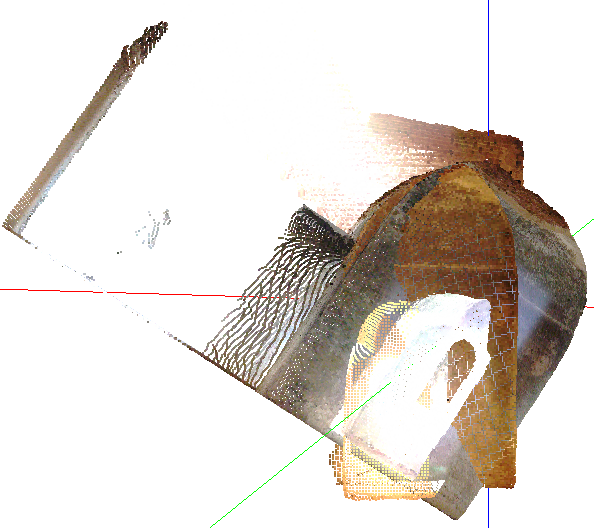
\includegraphics[width=0.7\linewidth]{/Más-ejemplos/sens-3_11} 
		%\label{fig:subim1}
	\end{minipage}
	\begin{minipage}[b]{0.5\textwidth}
		\centering
		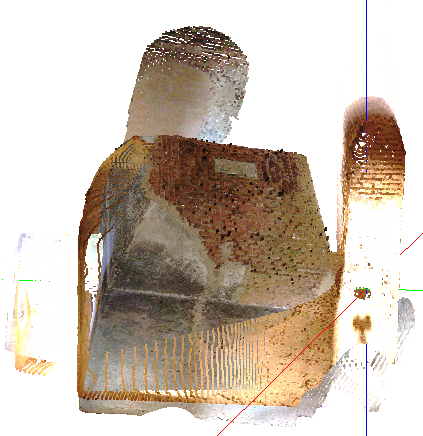
\includegraphics[width=0.7\linewidth]{/Más-ejemplos/sens-3_12}
		%\label{fig:subim2}
	\end{minipage}	
	\caption{Tras una iteración. Usamos un prealineado no exacto.}
	\label{fig:sensi-2-2}
\end{figure}

\begin{figure}[h!]	
	\begin{minipage}[b]{0.5\textwidth}
		\centering		
		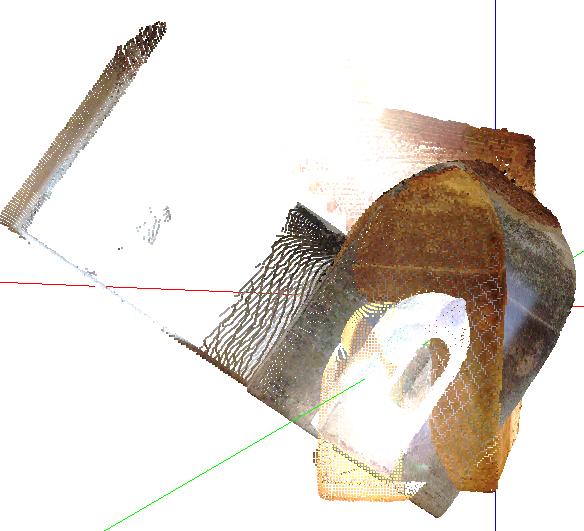
\includegraphics[width=0.7\linewidth]{/Más-ejemplos/sens-3_21} 
		%\label{fig:subim1}
	\end{minipage}
	\begin{minipage}[b]{0.5\textwidth}
		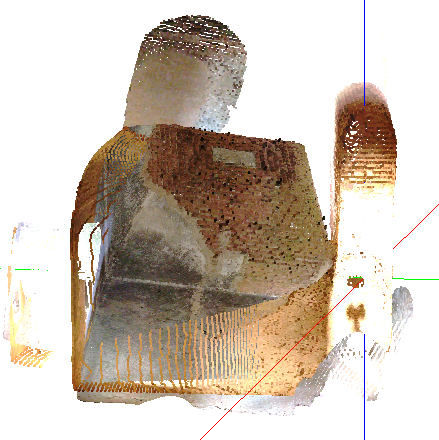
\includegraphics[width=0.7\linewidth]{/Más-ejemplos/sens-3_22}
		%\label{fig:subim2}
	\end{minipage}	
	\caption{Tras dos iteraciones. Usamos un prealineado no exacto.}
	\label{fig:sensi-2-3}
\end{figure}

Vemos, que como en el anterior, el modelo apenas cambia tras aplicarle el algoritmo. Finalmente, realizamos el proceso con un prealineado un poco más fino que el anterior. Este proceso aparece reflejado en las figuras \ref{fig:sensi3-1}, \ref{fig:sensi3-2} y \ref{fig:sensi3-3}.\\

En este caso, hemos tardado 6 iteraciones en conseguir un resultado que podríamos considerar satisfactorio. No es tan preciso como en la sección anterior cuando el prealineado era mejor, pero teniendo en cuenta la situación inicial lo podemos considerar como aceptable. Por ejemplo, si nos fijamos en la evolución de las fotos de la izquierda, observamos cómo la esquina inferior se va a acercando cada vez más entre ambas tomas hasta estar bastante cercana en ambos casos

\begin{figure}[h!]	
	\begin{minipage}{0.5\textwidth}
		\centering		
		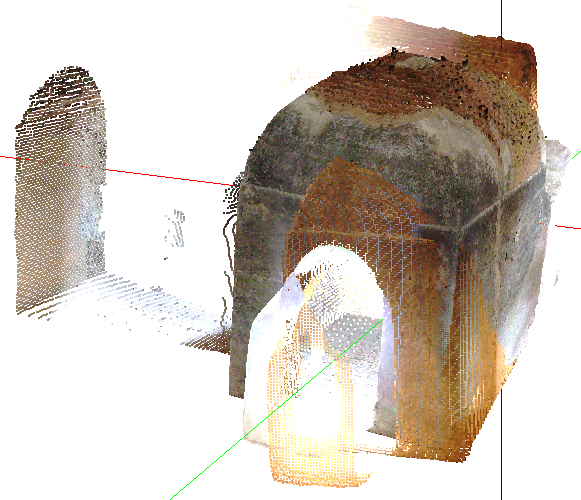
\includegraphics[width=0.8\linewidth]{/Más-ejemplos/sens-2_01} 
		%\label{fig:subim1}
	\end{minipage}
	\begin{minipage}{0.5\textwidth}
		\centering
		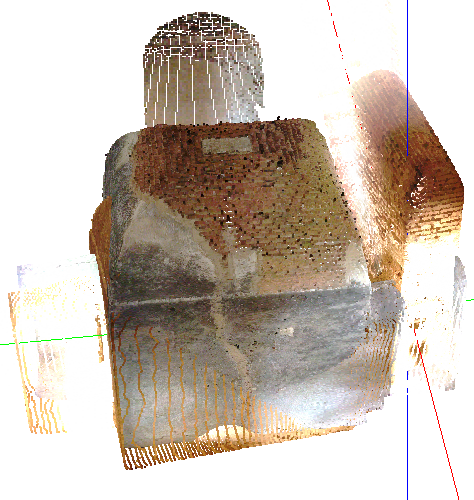
\includegraphics[width=0.8\linewidth]{/Más-ejemplos/sens-2_02}
		%\label{fig:subim2}
	\end{minipage}	
	\caption{Situación inicial. Las tomas están mejor prealineadas.}
	\label{fig:sensi3-1}
\end{figure}
\begin{figure}[h!]	
	\begin{minipage}{0.5\textwidth}
		\centering		
		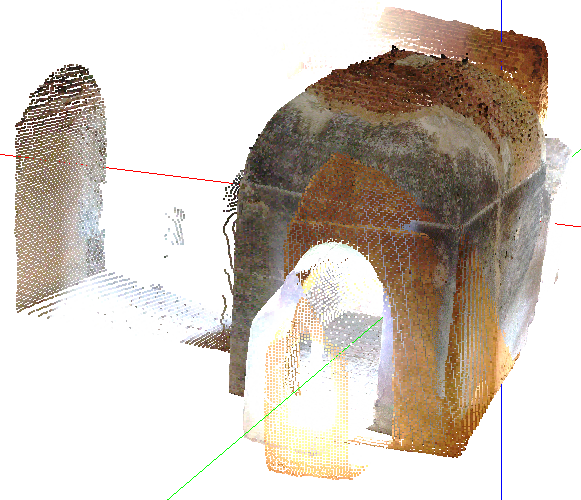
\includegraphics[width=0.8\linewidth]{/Más-ejemplos/sens-2_11} 
		%\label{fig:subim1}
	\end{minipage}
	\begin{minipage}{0.5\textwidth}
		\centering
		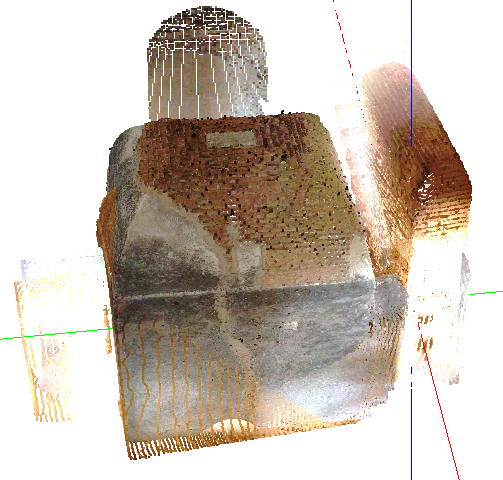
\includegraphics[width=0.8\linewidth]{/Más-ejemplos/sens-2_12}
		%\label{fig:subim2}
	\end{minipage}	
	\caption{Tras una iteración. Las tomas están mejor prealineadas.}
	\label{fig:sensi3-2}
\end{figure}
\begin{figure}[h!]	
	\begin{minipage}{0.5\textwidth}
		\centering		
		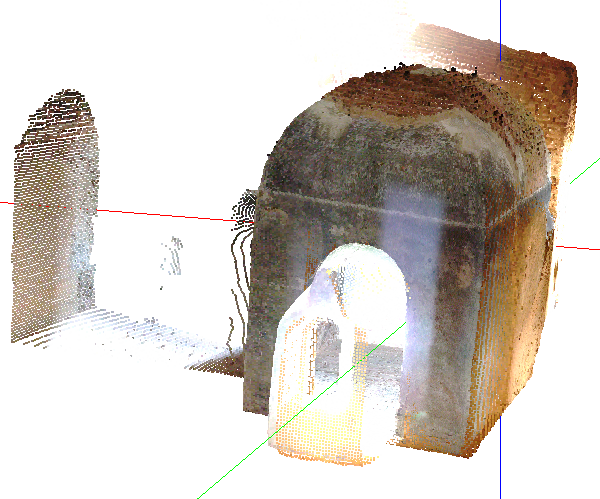
\includegraphics[width=0.8\linewidth]{/Más-ejemplos/sens-2_61} 
		%\label{fig:subim1}
	\end{minipage}
	\begin{minipage}{0.5\textwidth}
		\centering
		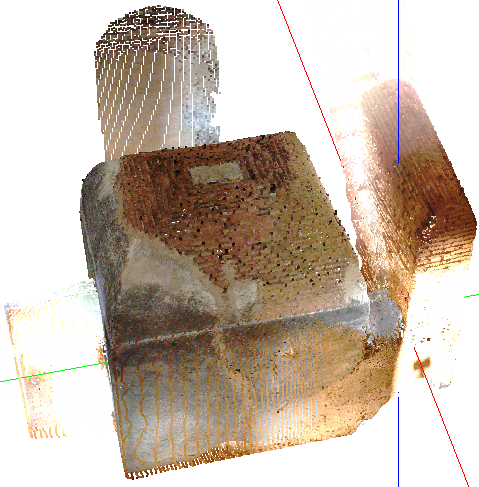
\includegraphics[width=0.8\linewidth]{/Más-ejemplos/sens-2_62}
		%\label{fig:subim2}
	\end{minipage}	
	\caption{Tras seis iteraciones. Las tomas están mejor prealineadas.}
	\label{fig:sensi3-3}
\end{figure}


\section{Conclusiones}
Concluimos el estudio del algoritmo ICP con una sección de conclusiones acerca de todo lo que hemos visto hasta ahora. En primer lugar, gracias a este procedimiento hemos conseguido un  mecanismo para alinear dos nubes correspondientes a un mismo objeto. Para poder comprenderlo hemos tenido que realizar un estudio previo acerca de los cuaternios. Sin embargo, este algoritmo tiene una convergencia local lo que significa que ambas tomas deben estar los suficientemente ``cerca'' una de otra para obtener una solución adecuada. Esta situación hace necesario el uso de un prealineado inicial e incluso haciendo uso de él puede que no consigamos un resultado satisfactorio. Otro inconveniente que presenta es la complejidad cuadrática en tiempo. Esto implica que hasta en modelos simples, tarde bastante tiempo en completarse cada una de las iteraciones. Por ello, para intentar acelerar el proceso hemos introducido unos descriptores para cada uno de los puntos basándonos en la variación de la normal. Esto ha sido posible gracias a la forma que tiene el escáner usado para la realización de tomas de darnos los resultados. De esta forma hemos detectado zonas significativas en ambas tomas  y realizado el mecanismo de alineación entre ellas. Hemos podido comprobar que los resultados han sido satisfactorios teniendo en cuenta tanto la simplificación del modelo para la obtención de las normales como el hecho de usar una parte de cada una de las nubes de puntos en el procedimiento.